% Author: Nikitha Jayant Bangera
% Version: 1.0

\documentclass[12pt, a4paper]{report}
\usepackage[left=2.5cm, right=2.5cm, top=1cm, bottom=1.5cm]{geometry}
\usepackage[utf8]{inputenc}
\usepackage{amssymb}
\usepackage{amsmath}
\usepackage{latexsym}
\usepackage[normalem]{ulem}
\usepackage{array}
\usepackage{graphicx, tabularx}
\usepackage[backend=biber,
style=numeric,
sorting=none,
isbn=false,
doi=false,
url=false,
]{biblatex}\addbibresource{bibliography.bib}
\usepackage{biblatex}
\usepackage{array,multirow}
\usepackage{longtable}

\date{}

\title{
\includegraphics[width=10cm,height=5cm]{Con_Logo1.jpg}\\\\}
\author{
\LARGE{Eternity: Numbers}
\\\\
A project report presented for the course\\ 
SOEN 6481 \\\textit{Software Requirements Specifications}
\\ \\ 
\\ \Large{Author Name}
\\ Nikitha Jayant Bangera
\\\\ \\
Under the guidance of\\
Professor Pankaj Kamthan
}
%%%%%%%%%%%%%%%%%%%%%%%%%%%%%%%%%%%%%%%%%%%%%%%%%%%%%%%%%%%%%%%%%%%%%%%
\begin{document}
\thispagestyle{headings}
	\maketitle
\pagenumbering{roman}

\thispagestyle{empty}
\chapter*{Acknowledgements}
I would like to express my sincere thanks to Professor Pankaj Kamthan for his advice and encouragement throughout the First deliverable of the Eternity: Numbers project, as well as to my Technical Lab Assistant for his guidance throughout the first phase of the project. 
\thispagestyle{empty}
\begin{abstract}
%\lipsum[1-2]
The document tries to put some light on the understanding of an irrational number, The Champernowne Constant. A brief description of the constant and some of its applications are included in the report. A research and interview on the constant was conducted with a resource who is familiar with Champernowne constant. My interviewee tried to answer most common questions about the constant in a questionnaire that also describes some applications of Champernowne constant. Based on the understanding of Champernowne Constant, a calculator application is to be built, that uses this constant to perform certain operations. This document also gives the basic design details on how the product would look like,what operations is it capable of, its algorithm and use cases.
\end{abstract}

\tableofcontents
\thispagestyle{plain}
\listoffigures
\listoftables

\chapter{Use Case Model}
\pagenumbering{arabic}
\section{UML Use Case Diagram}
\quad The following diagram shows the use case view of Eternity Numbers calculator for Champernowne Constant followed by the Activity diagram and sequence diagrams in sections 5.2 and 5.3

\begin{figure}[h]
    \centering
    \fbox{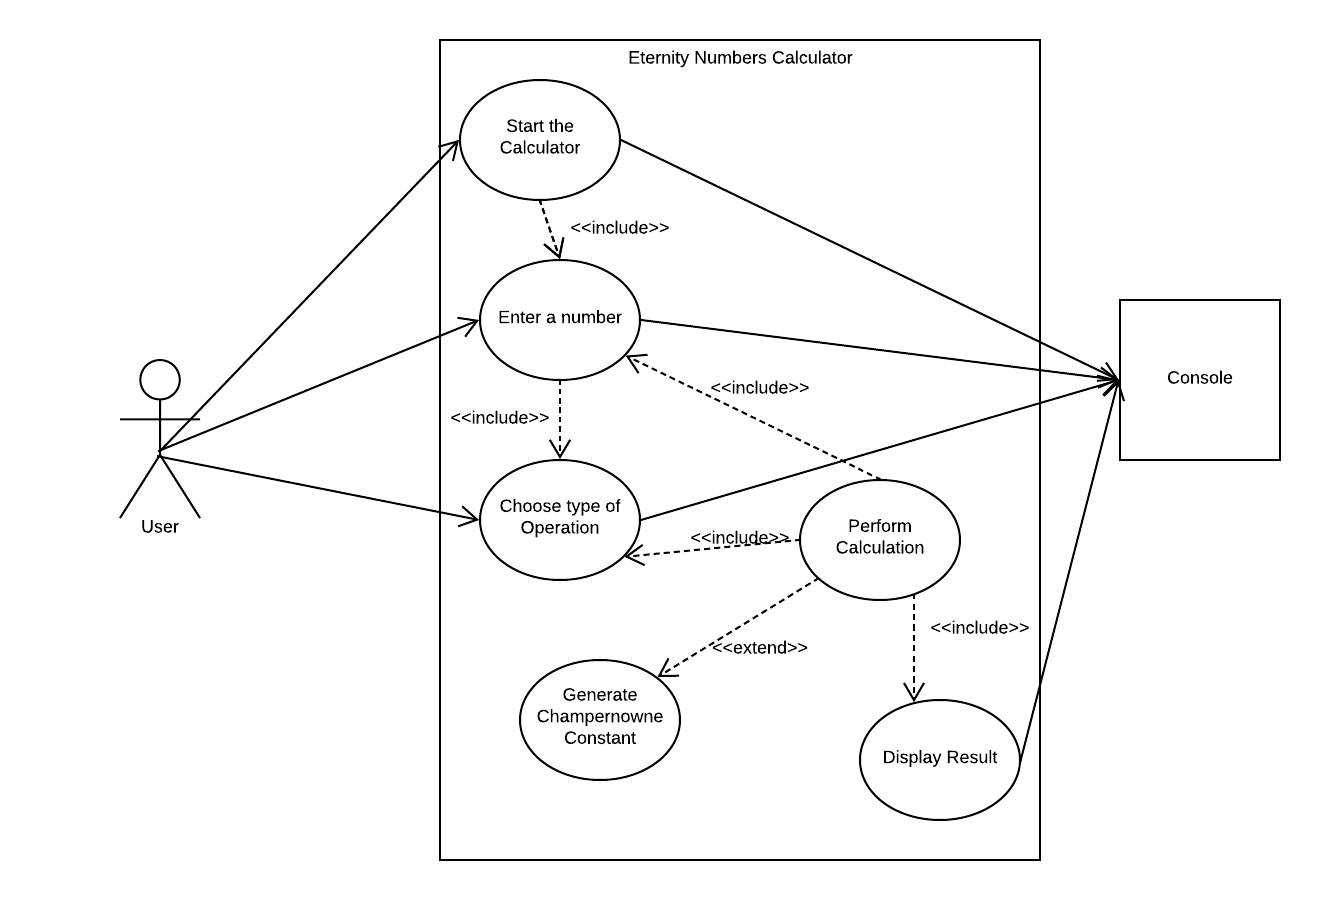
\includegraphics[width=160mm, height=100mm]{ChampernowneUseCase.png}}
    \caption{UML Use Case diagram of Eternity: Numbers}
    \label{fig:UML Use Case diagram of Eternity: Numbers}
\end{figure}

Steps in the Use case model of Eternity numbers calculator (Refer to Figure 5.1):
\begin{enumerate}

    \item User starts the calculator application i.e. Eternity: Numbers calculator. The application displays a set of operations , which a user can pick to perform various operations.
    \item User selects the required operation like addition, subtraction, finding a position of a number in Champernowne Constant, Generating a Champernowne Constant etc.
    \item The applications prompts the user to enter required input values to perform the opetation.
    \item User enters the number.
    \item The system processes user's input and displays results to the user.
\end{enumerate}
\section{UML Activity Diagram}
Figure 1.2 shows the Activity diagram representation of the above use case. If the user selects any other constant other than the Champernowne constant, a relevant message is displayed that the feature is not available as this version of the product focuses on Champernowne Constant only.\\\\
%\hspace{15mm}
\begin{figure}[!h]
    \centering
    \fbox{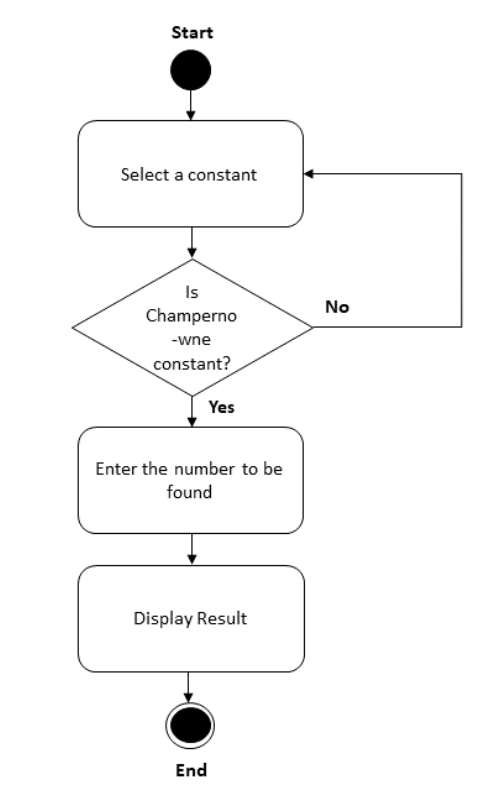
\includegraphics[width=50mm, height=70mm]{ChampernowneActivity.PNG}}
    \caption{UML Activity diagram of Eternity: Numbers}
    \label{fig:UML Activity diagram of Eternity: Numbers}
\end{figure}

\section{Sequence diagram}
Figure 1.3 shows the sequence diagram of the Eternity Numbers caculator application
\begin{figure}[h]
    \centering
    \fbox{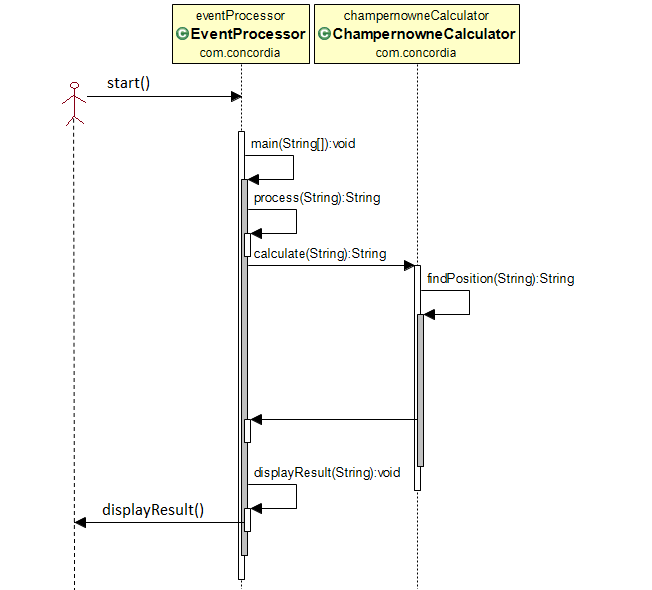
\includegraphics[width=100mm, height=80mm]{EternityNumbersSequenceDiagram.png}}
    \caption{UML Sequence diagram of Eternity: Numbers}
    \label{fig:UML Sequence diagram of Eternity: Numbers}
\end{figure}

\section{Normal Scenario of Use case model}
\quad The following section explains all 6 use cases depicted in Fig.1.1 and are described below with sequence diagrams for all the use cases. The sequence diagram explains a single thread view of the application.
\subsection{Use Case 1 - Start(UC001)}
\quad The user starts the calculator application, The calculator application will Display a set of messages on the console/user screen prompting user with the options to proceed further.
\begin{figure}[h]
    \centering
    \fbox{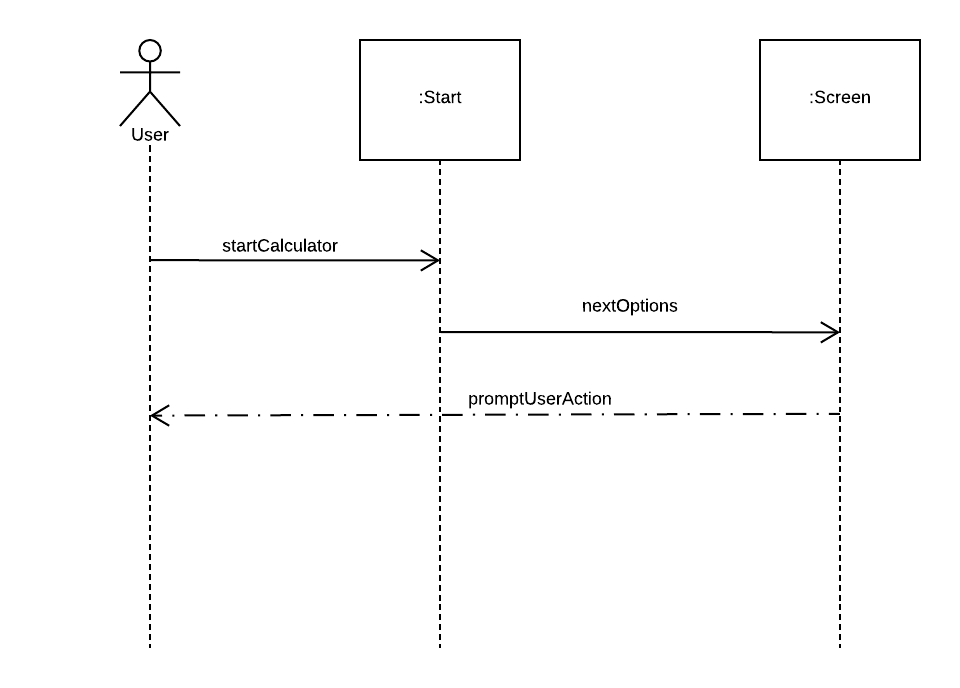
\includegraphics[width=80mm, height=50mm]{UseCase1.png}}
    \caption{UC001 Start Calculator}
    \label{fig:UC001 Start Calculator}
\end{figure}

\subsection{Use Case 2 - Enter a number(UC002)}
\quad The user enters the random number that will be used for the calculations. The calculator application will accept the input and display options on screen for user to proceed further.
\begin{figure}[!h]
    \centering
    \fbox{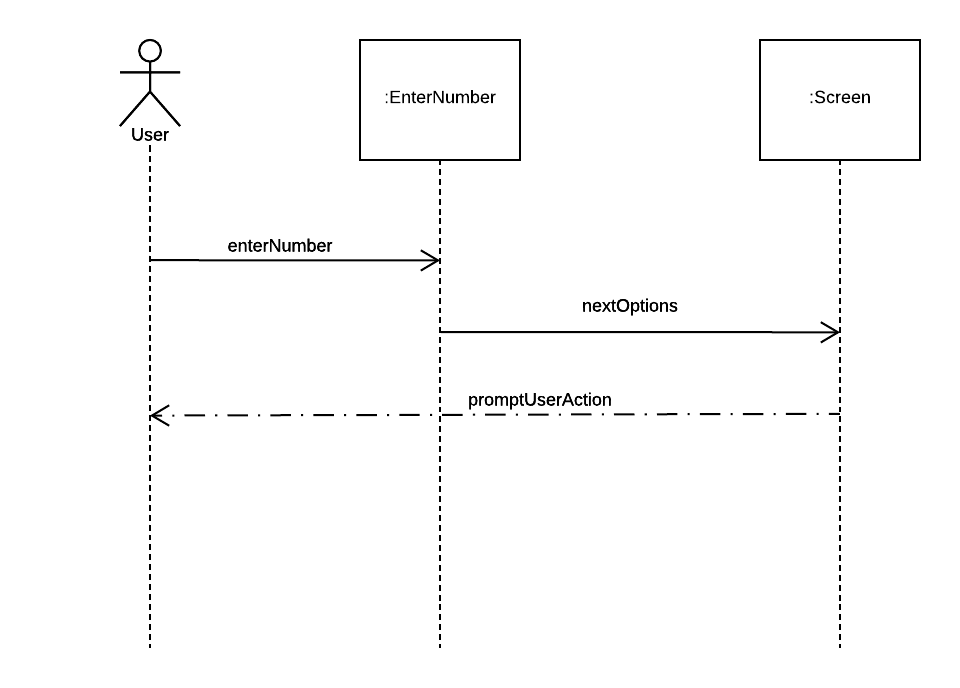
\includegraphics[width=80mm, height=50mm]{UseCase2.png}}
    \caption{UC002 Enter Number}
    \label{fig:UC002 Enter Number}
\end{figure}

\subsection{Use Case 3 - Choose type of Operation(UC003)}
\quad The user selects one of the options which is read by the calculator and starts processing the request or prompts user with messages if any other inputs are needed.\\\\
\begin{figure}[h]
    \centering
    \fbox{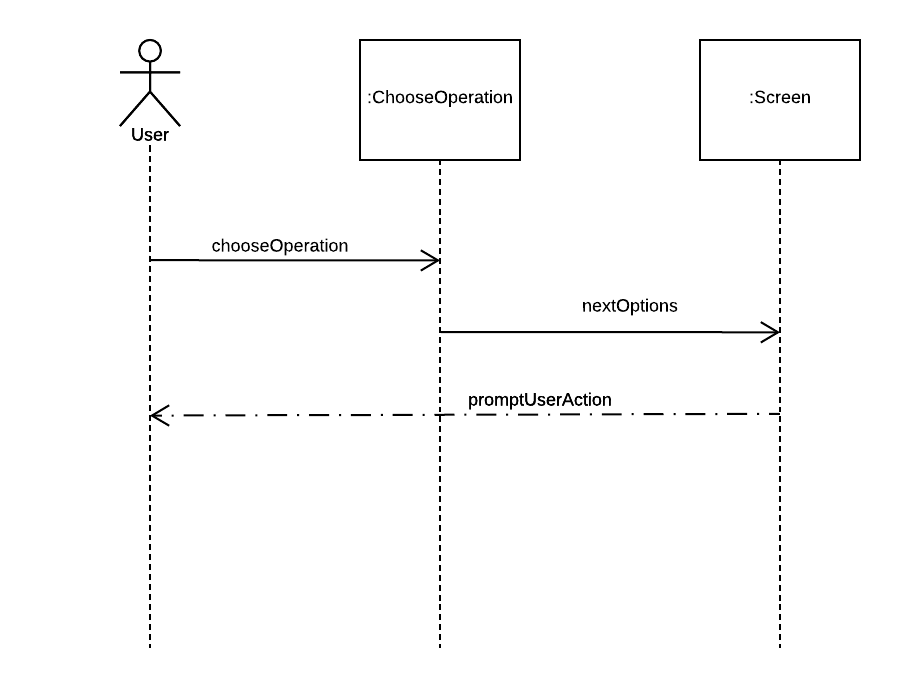
\includegraphics[width=100mm, height=80mm]{UseCase3.png}}
    \caption{UC003 Choose Type of Operation}
    \label{fig:UC003 Choose Type of Operation}
\end{figure}

\subsection{Use Case 4 - Perform Calculation(UC004)}
\quad The request opted from the user is picked up for processing and the calculator invokes relevant operation to process the data.
\begin{figure}[h]
    \centering
    \fbox{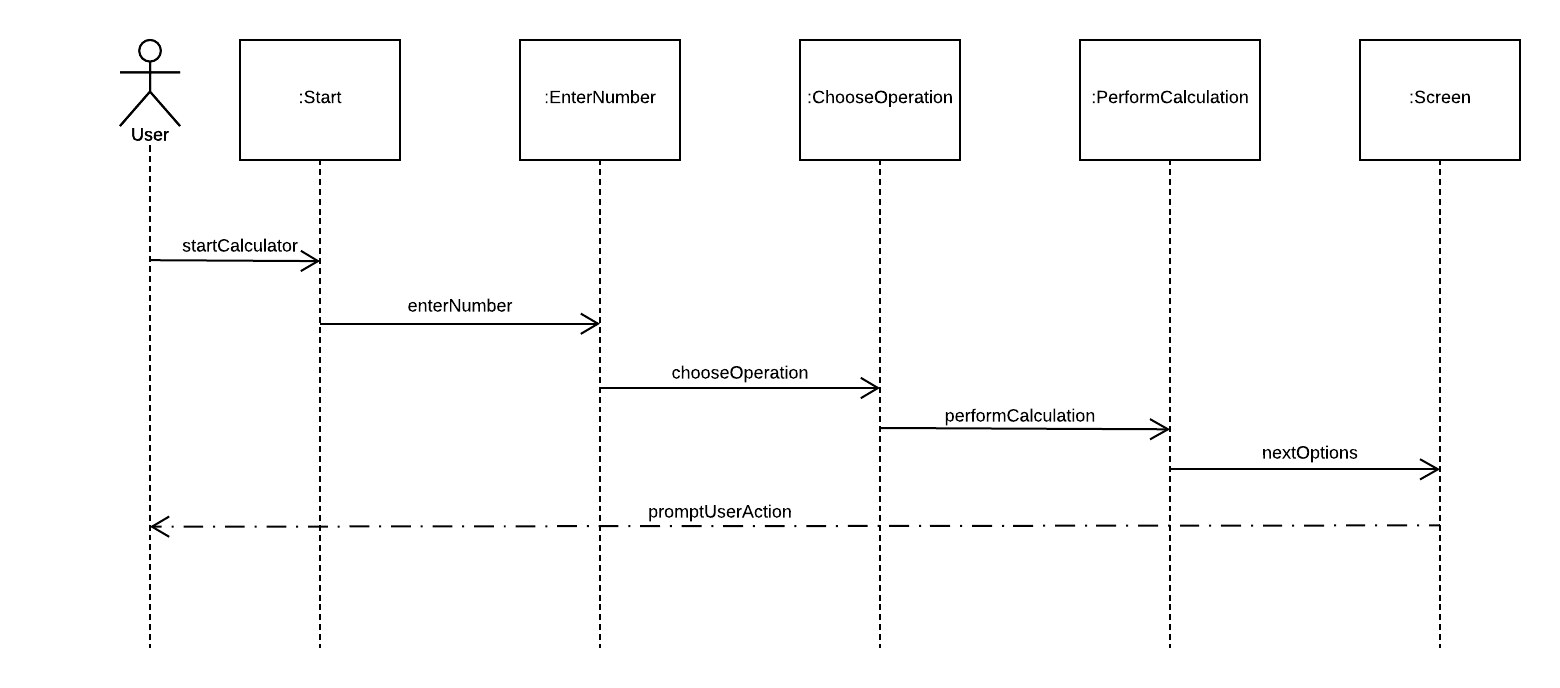
\includegraphics[width=140mm, height=80mm]{UseCase4.png}}
    \caption{UC004 Perform Calculation}
    \label{fig:UC004 Perform Calculation}
\end{figure}

\subsection{Use Case 5 - Generate Champernowne Constant}
\quad This is an extension of Perform Calculation which is invoked when the user selects one of the options to generate the Champernowne Constant.\\\\
\begin{figure}[h]
    \centering
    \fbox{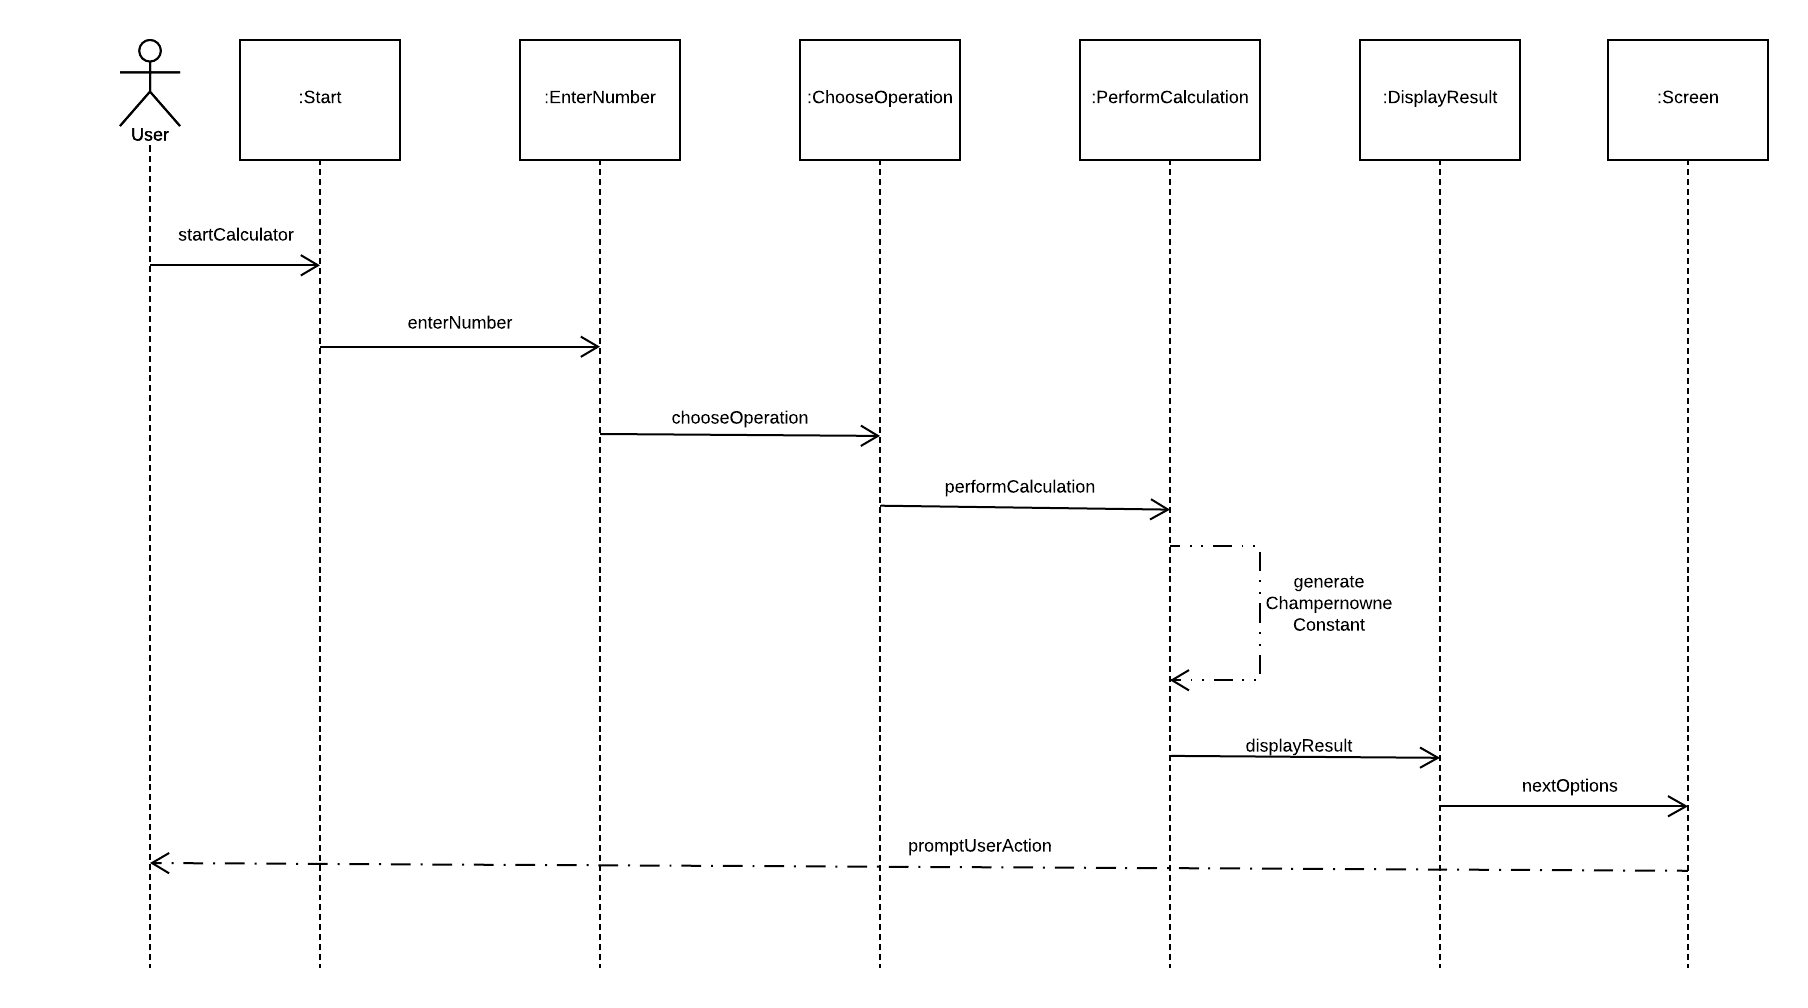
\includegraphics[width=160mm, height=80mm]{UseCase5.png}}
    \caption{UC005 Generate Champernowne Constant}
    \label{fig:UC005 Generate Champernowne Constant}
\end{figure}

\subsection{Use Case 6 - Display Result(UC006)}
\quad The results of the calculations performed based on user's choice are streamed to the console to be displayed to the user.
\begin{figure}[h]
    \centering
    \fbox{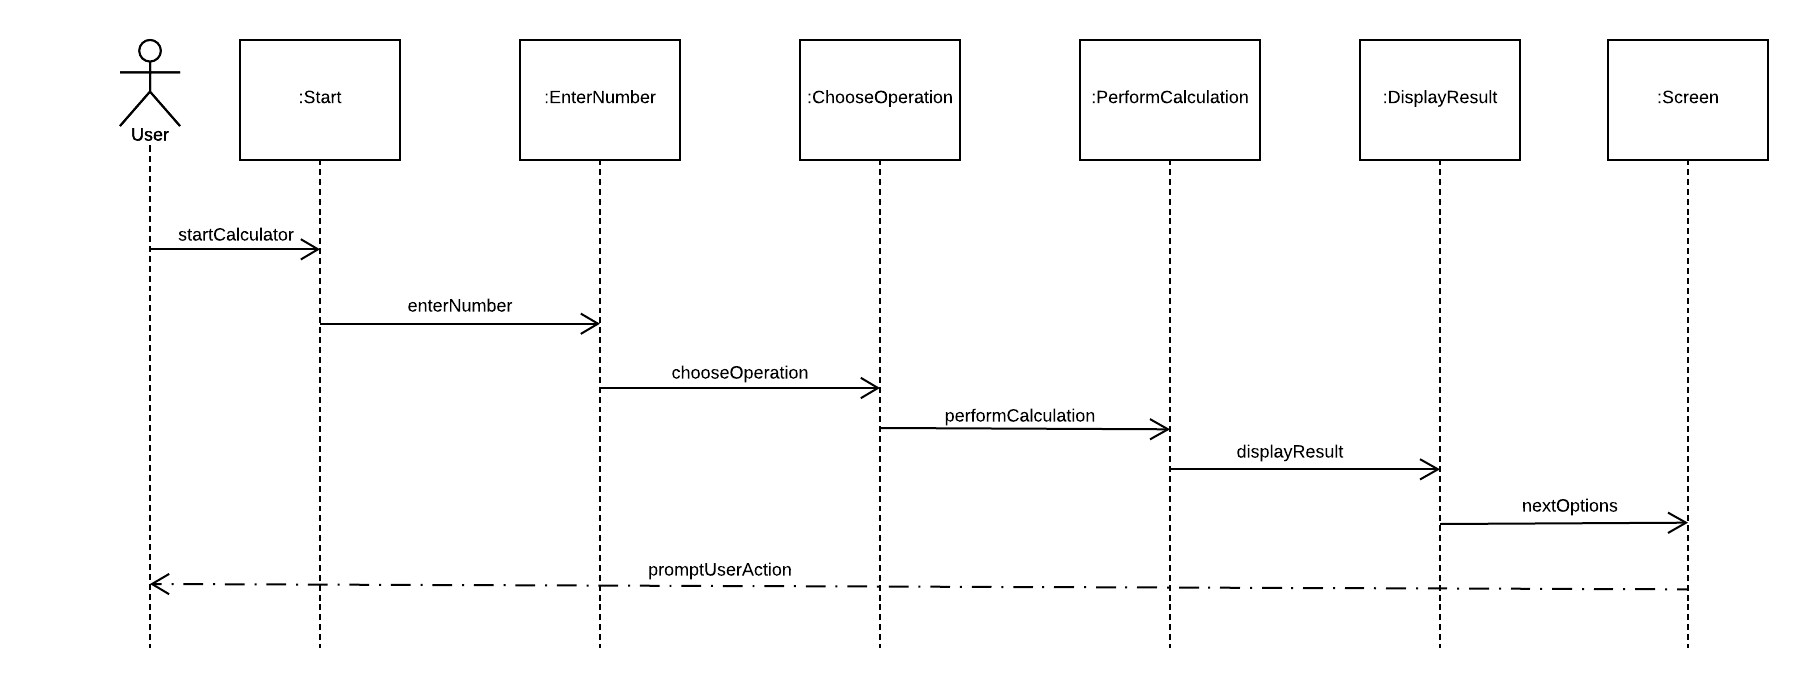
\includegraphics[width=160mm, height=80mm]{UseCase6.png}}
    \caption{UC006 Display Result}
    \label{fig:UC006 Display Result}
\end{figure}



\chapter{User stories and Traceability Matrix}
\section{User stories and Acceptance Test cases}
The following table describes the list of user stories and acceptance test cases for every user story.
\\\\
\begin{tabular}{|p{3cm}|p{12cm}|}
\hline
     \textbf{US001} &  As a user, I want to find the position of a given number in the sequence of positive integers to calculate the total number of digits between 0 and the given number.\\\hline
     \textbf{Constraint} &  \textbf{1. } The input number cannot be a decimal or a negative number as the champernowne constant is a series of positive integers at base 10. \newline \textbf{2. } The number entered should always be numeric.\\\hline
     \textbf{Priority} & 5 \\\hline
     \textbf{Estimate} & 1 \\\hline
     \multirow{2}{3cm}{\textbf{Acceptance Test cases}} & \textbf{TC001} - Start the calculator application. Enter a random positive integer number as 100. Select "Find Position in Champernowne Constant" from the options menu. \newline \textbf{Output} - The position of number 100 in Champernowne Constant(C10) is 190.\\\cline{2-2}
     & \textbf{TC002} - Start the calculator application. Enter a random String as "abc". \newline \textbf{Output} - Please enter a valid positive integer number.\\\cline{2-2}
     & \textbf{TC003} - Start the calculator application. Enter a random positive decimal number. Select "Find Position in Champernowne Constant" from the options menu. \newline \textbf{Output} - Please enter a valid positive integer number.\\\hline
\end{tabular}
\\\\\\
\begin{tabular}{|p{3cm}|p{12cm}|}
\hline
     \textbf{US002} &  As a user, I want to save the random number entered by user and find its square value to display a message "The square of X is Y".\\\hline
     \textbf{Constraint} &  \textbf{1. } The number entered to calculate the square should always be numeric.\\\hline
     \textbf{Priority} & 4 \\\hline
     \textbf{Estimate} & 2 \\\hline
     \multirow{2}{3cm}{\textbf{Acceptance Test cases}} & \textbf{TC004} - Start the calculator application. Enter a random positive integer number as 3. Select "Save the number". Select "Find the square of the number". \newline \textbf{Output} - "The square of \textbf{3} is \textbf{9}"\\\cline{2-2}
     & \textbf{TC005} - Start the calculator application. Enter a random positive decimal number. Select "Find Position in Champernowne Constant" from the options menu. \newline \textbf{Output} - Please enter a valid positive integer number.\\\hline
\end{tabular}
\\\\\\\\
\\
\begin{tabular}{|p{3cm}|p{12cm}|}
\hline
     \textbf{US003} &  As a user, I want to calculate the Champernowne constant to generate the sequence of incremental positive numbers.\\\hline
     \textbf{Constraint} &  \textbf{1. } The input number cannot be a decimal or a negative number as the champernowne constant is a series of positive integers at base 10. \newline \textbf{2. } The number entered should always be numeric.\\\hline
     \textbf{Priority} & 3 \\\hline
     \textbf{Estimate} & 4 \\\hline
     \multirow{2}{3cm}{\textbf{Acceptance Test cases}} & \textbf{TC006} - Start the calculator application. Enter a random positive integer number as 12. Select "Generate Base 10 Champernowne Constant". \newline \textbf{Output} - The calculator application should display the message "The Base 10 Champernowne constant of length \textbf{12} digits is \textbf{0.123456789101}.\\\cline{2-2}
     & \textbf{TC007} - Start the calculator application. Enter a random positive decimal number. Select "Find Position in Champernowne Constant" from the options menu. \newline \textbf{Output} - Please enter a valid positive integer number.\\\hline
\end{tabular}
\\\\\\\\
\begin{tabular}{|p{3cm}|p{12cm}|}
\hline
     \textbf{US004} &  As a user, I want to generate random binary digits to use the random sequence to enable/disable relay switches.\\\hline
     \textbf{Constraint} &  \textbf{1. } The input number cannot be a decimal or a negative number as the champernowne constant is a series of binary digits at base 2. \newline \textbf{2. } The number entered should always be numeric.\\\hline
     \textbf{Priority} & 2 \\\hline
     \textbf{Estimate} & 8 \\\hline
     \multirow{2}{3cm}{\textbf{Acceptance Test cases}} & \textbf{TC008} - Start the calculator application. Enter a random positive integer number. Select "Generate Binary Champernowne constant". \newline \textbf{Output} - The Base 2 Champernowne constant of length \textbf{12} digits is \textbf{0.110111001011}\\\cline{2-2}
     & \textbf{TC009} - Start the calculator application. Enter a random positive decimal number. Select "Find Position in Champernowne Constant" from the options menu. \newline \textbf{Output} - Please enter a valid positive integer number.\\\hline
\end{tabular}
\\\\\\\\
\begin{tabular}{|p{3cm}|p{12cm}|}
\hline
     \textbf{US005} &  As a user, I want to find the positions of two different numbers in a sequence of positive integers to identify the number of digits between the two numbers.\\\hline
     \textbf{Constraint} &  \textbf{1. } The input number cannot be a decimal or a negative number as the champernowne constant is a series of positive integers at base 10. \newline \textbf{2. } The number entered should always be numeric.\\\hline
     \textbf{Priority} & 1 \\\hline
     \textbf{Estimate} & 16 \\\hline
     \multirow{2}{3cm}{\textbf{Acceptance Test cases}} & \textbf{TC010} - Start the calculator application. Enter a random positive integer number 10. Select "Find the position of the Number in Champernowne Constant". Select "Save the Number". Select "Find the square of a Number". Select "Find the position of the number in Champernowne Constant". Select "Previous Number". Select "Subtraction" between "Previous result" and  "Saved Number". \newline \textbf{Output} - The difference of \textbf{190} and \textbf{10} is \textbf{180}. \newline \textbf{Note}: 190 is the starting position of number 100(Square of 10 in this case) and 10 is the starting position of 10  \\\cline{2-2}
     & \textbf{TC011} - Start the calculator application. Enter a random positive decimal number. Select "Find Position in Champernowne Constant" from the options menu. \newline \textbf{Output} - Please enter a valid positive integer number.\\\hline
\end{tabular}starting 

\chapter {Backward Traceability Matrix}

\begin{longtable}{|p{1.5cm}|p{3cm}|p{2cm}|p{4cm}|}

    \hline
    User Stories & Use Cases & Persona & Requirements / Interview Questions \\\hline
    US001 & UC001, UC002, UC003, UC004, UC006 & X & 1,2,14\\\hline
    US002 & UC001, UC002, UC003, UC004, UC006 &NA &NA\\\hline
    US003 & UC001, UC002, UC003, UC004, UC005, UC006 & X & 14\\\hline
    US004 & UC001, UC002, UC003, UC004, UC005, UC006 & X & 10\\\hline
    US005 & UC001, UC002, UC003, UC004, UC005, UC006 & X & 1,2,14\\\hline
\caption{Table for Backward Traceability Matrix}
\label{table:1}
\end{longtable}
{*Refer Figure 2.1 for the User Stories and Figure 1.1 for the Use Case Diagram.}
\\
\chapter{Eternity:Numbers Calculator}

\section{Generic Guidelines}

\quad To launch the Eternity:Numbers calculator application, please follow the below steps - 

\begin{itemize}
    \item Download the source code from the git repository \newline \underline{https://github.com/NikithaBangera/SOEN6481Project}
    \item Open Eclipse,
    \item Select File, and choose Open Project from FileSystem,
    \item Browse to the location where you downloaded the .zip file from the git repository,
    \item Select the project folder and click Ok,
    \item Open the EternityNumber.java file,
    \item Right click anywhere in the window and Select Run As - Java Application.
\end{itemize} 

\section{Guidelines for User Stories}

\subsection{User Story 1(US001)}
\begin{itemize}
    \item The calculator application prompts to enter a number,
    \item Enter a number 100 and hit enter,
    \item Now enter 8, to select Option "8.Find the position in Champernowne Constant(C10)" and hit enter,
    \item The calculator application will display a message "The position of 100 in Champernowne constant(C10) is 190.
\end{itemize}

\subsection{User Story 2(US002)}
\begin{itemize}
    \item The calculator application prompts to enter a number,
    \item Enter a number 10 and hit enter,
    \item Now enter 6, to select Option "6. Square of a number" and hit enter,
    \item The calculator application will display a message "The square of 10 is 100".
\end{itemize}

\subsection{User Story 3(US003)}
\begin{itemize}
    \item The calculator application prompts to enter a number,
    \item Enter a number 12 and hit enter,
    \item Now enter 10, to select Option "10. Generate base 10 Champernowne Constant(C10)" and hit enter,
    \item The calculator application will display a message "The base 10 Champernowne constant of length 12 digits is 0.123456789101.
\end{itemize}

\subsection{User Story 4(US004)}
\begin{itemize}
    \item The calculator application prompts to enter a number,
    \item Enter a number 12 and hit enter,
    \item Now enter 9, to select Option "9. Generate a binary Champernowne constant(C2)" and hit enter,
    \item The calculator application will display a message "The base 2 Champernowne constant of length 12 digits is 0.110111001011.
\end{itemize}

\subsection{User Story 5(US005)}
\begin{itemize}
    \item The calculator application prompts to enter a number,
    \item Enter a number 10 and hit enter,
    \item Now enter 8, to select Option "8. Find the position in Champernowne Constant(C10)" and hit enter,
    \item The calculator application will display a message The calculator application will display a message "The position of 10 in Champernowne constant(C10) is 10.
    \item Now enter 11, to select Option "11. Save the number" and hit enter,
    \item The calculator application should display the message "Number 10 saved successfully."
    \item Now enter 6, to select Option "6. Square of a number" and hit enter,
    \item The calculator application will display options to select which number to choose to calculate the square value.
    \item Now enter 1, to select Option "1.Saved Number" and hit enter.
    \item The calculator application should display the message "The square of 10 is 100.0"
    \item Now enter 8, to select Option "8. Find the position in Champernowne Constant(C10)" and hit enter
    \item The calculator application will display options to select which number to choose to proceed further.
    \item Now enter 2, to select Option "2.Previous Result" and hit enter
   \item The calculator application should display the message "The position of 100 in Champernowne constant(C10) is 190"
   \item Now enter 2, to select option "2. Subtraction" and hit enter,
   \item The calculator application will display options to select which number to choose as first number for subtraction.
   \item Now enter 2, to select Option "2.Previous Result" and hit enter
    \item The calculator application will display options to select which number to choose as Second number for subtraction.
    \item Now enter 1, to select Option "1.Saved Number" and hit enter.
    \item The calculator application should display a message "The difference of 190 and 10 is 180"
    
\end{itemize}

\chapter{Version Control Repository}
The link for my Github Repository is given below:\\
\url{https://github.com/NikithaBangera/SOEN6481Project}

\begin{thebibliography}{9}
    \bibitem {Wikipedia}
    \texttt{https://en.wikipedia.org/wiki/Champernowne{\_}constant}
    \bibitem {Wolfram}
    \texttt{http://mathworld.wolfram.com/ChampernowneConstant.html}
    \bibitem{wikia}
    \texttt{https://googology.wikia.org/wiki/Champernowne{\_}constant{\_}continued{\_}fraction}
    \bibitem {FSE}
    \texttt{http://fse.studenttheses.ub.rug.nl/}
    \bibitem {Online Encyclopedia Champernowne constant base 10}
    \texttt{https://oeis.org/A065649}
    \bibitem {An Interesting property of Champernowne's number}
    \texttt{https://www.kanonical.io/an{\_}interesting{\_}property{\_}of{\_}champernownes{\_}number/}
\end{thebibliography}
\end{document}

